% ===== Multimodal indirect-feedback RAG (Experiment: mm-RAG) =====
% PROVISIONAL DRAFT — numbers under main-session review; do not merge into the main text
% until the review passes. Evidence pointers: VLM2Vec-in repo, mmrag/RESULTS.md +
% results_summary.json (run name -> job id -> checkpoint), mmrag/REPRO_NEWCLUSTER.md
% (independent-hardware reproduction), checkpoints at huggingface.co/Icey444/mmrag-ckpts.
\subsection{Multimodal: retriever RL from VLM answer success}
\label{sec:mm_rag}
We port the indirect-feedback recipe to knowledge-VQA: the retriever is
\textsc{GME-Qwen2-VL-2B} (LoRA), queries are image--question pairs (InfoSeek), the corpus is a
422K-passage Wikipedia KB, and the reward is a frozen \textsc{Qwen2.5-VL-3B} reader's sampled
answer accuracy on the retrieved passage (cover-EM vs.\ official aliases, $4$ rollouts, per-pool
z-scored), with GRPO on top-$N{=}8$ pools and an InfoNCE anchor.

\paragraph{Annotation-free RL works in multimodal.} Unlike the text setting, where [no-gold]
training never exceeded its zero-shot base, the multimodal [no-gold] arm --- pools are purely the
policy's own retrievals; the \emph{only} supervision is the gold answer inside the reward ---
beats both zero-shot ($34.1$ vs.\ $30.3$ VQA accuracy) and the LR-tuned relevance-SFT baseline
($32.1$; paired McNemar $p{=}0.024$, replicated across seeds), and is statistically
indistinguishable from gold-seeded pools ($p{=}0.93$). Neither deterministic nor sampled
[no-gold] pools collapse. At 7B the picture strengthens: zero-shot $30.6$ $\to$ SFT $32.6$
$\to$ indirect RL $35.9$ ([no-gold]: $35.1$, $p{=}1.3\mathrm{e}{-7}$ vs.\ zero-shot), so the
indirect-feedback advantage again grows with retriever capacity, while at the CLIP/SigLIP rungs
SFT wins --- the same capacity dichotomy as in text.

\paragraph{The reward source, benchmarked through one loop.} Swapping only the reward:
relevance labels as reward (\emph{goldrel}) reach $31.7$ on [no-gold] pools --- \emph{below} the
reader reward ($34.1$) --- because the oracle signal is sparse on policy pools; a lexical
answer-match reward reaches $33.4$. The reader's dense-sampling accuracy is the best-shaped
signal, and a 3B reward reader matches a served 7B one ($33.7$ vs.\ $34.1$). Binary answer
accuracy is \emph{required} here: the dense log-likelihood reward fails on [no-gold] pools
($31.5$), inverting the text-side preference. Slate-level rewards (accuracy over the joint
top-$k$ context) destabilize training and transfer catastrophically.

\paragraph{Reproduction on independent hardware.} The full pipeline was rebuilt from public
sources on a different cluster and re-run end to end. The rebuild recovers the corpus and query
counts exactly ($1{,}421{,}665$ / $422{,}378$ passages, $26{,}454$ articles, $45{,}248$ train /
$71{,}335$ test queries), so the comparison is like-for-like. Every arm reproduces within
$0.002$ absolute: zero-shot $30.80$ (recorded $31.00$), relevance-SFT $31.00$ (recorded $31.00$;
bit-identical on accuracy, strict-EM and F1), [no-gold] RL $33.93$ and $34.33$ for two seeds
(recorded $34.13$, $34.27$). The headline effect --- RL minus zero-shot --- reproduces exactly
at $+3.13$ points.

\paragraph{Does the gain generalize, or is it InfoSeek overfitting?}
Table~\ref{tab:mm_mmeb} evaluates all three arms on a fixed random subset of the MMEB image
tasks ($100$ queries $\times$ $37$ tasks, seed $0$, each task's full candidate pool retained).
One caveat determines how this must be read: MMEB's \textsc{OVEN} task draws its query images
from the same source as InfoSeek ($67$ of $100$ sampled OVEN images are in the InfoSeek image
store), so it is \emph{not} held out for our adapters; we therefore report the $36$-task macro
with OVEN removed as the primary number.
On genuinely held-out tasks the annotation-free adapter \emph{improves} general embedding
quality ($+0.83$ points over its base), while relevance-SFT is flat ($-0.03$). The
meta-task split shows why: SFT trades VQA-style embedding away (${-}2.10$, worse on $7$ of $10$
tasks and better on none) in exchange for classification ($+2.73$), whereas the indirect reward
--- which \emph{is} downstream answer success --- improves exactly the VQA-shaped capability
($+1.80$, better on $8$ of $10$). Neither arm shows the catastrophic forgetting reported for
in-domain contrastive fine-tuning of strong text embedders; we attribute this to the light
LoRA touch ($r{=}32$ on a frozen backbone) rather than to anything specific to the objective.

\begin{table}[t]
\centering\small
\caption{Generalization to MMEB image tasks after InfoSeek-only training. Macro Precision@1;
``excl.\ OVEN'' drops the one task whose images overlap InfoSeek. Meta-task deltas are versus the
zero-shot base, with (tasks better / worse) in parentheses.}
\label{tab:mm_mmeb}
\begin{tabular}{lccccc}
\toprule
& \multicolumn{2}{c}{macro P@1} & \multicolumn{3}{c}{$\Delta$ vs.\ base by meta-task} \\
\cmidrule(lr){2-3}\cmidrule(lr){4-6}
arm & all 37 & excl.\ OVEN & VQA & Classification & Retrieval \\
\midrule
zero-shot base   & 43.81 & 43.31 & --- & --- & --- \\
relevance-SFT    & 43.97 & 43.28 & $-2.10$ (0/7) & $+2.73$ (9/2) & $-0.75$ (4/6) \\
{}[no-gold] RL & \textbf{44.68} & \textbf{44.14} & $\mathbf{+1.80}$ (8/1) & $+1.09$ (8/2) & $-0.17$ (6/5) \\
\bottomrule
\end{tabular}
\end{table}

\paragraph{Neither more data nor more compute helps.} Holding the step budget fixed at $500$
steps and varying only the size of the training pool from $12.5$K to $200$K queries leaves
accuracy flat: $34.33$, $34.62{\pm}0.19$ (3 seeds), $34.67$, $32.87$, $34.80$. A $16\times$
increase in available training data buys nothing, and the whole ladder spans $2.0$ points while
the SFT-to-RL gap is $2.9$--$3.9$. The mechanism is a sampling ceiling: at $500$ steps
$\times$ batch $4$ the run visits only ${\sim}2{,}000$ queries regardless of pool size, so rows
beyond ${\sim}10$K are never sampled. Crucially this is \emph{not} a truncated compute curve ---
tripling the budget at fixed pool makes the model \emph{worse} ($34.13 \to 31.93$ at $41$K,
$34.07 \to 32.20$ at $8$K), so the recipe is already at or past its optimum. The replicated
three-seed cell at $25$K ($34.62{\pm}0.19$) sits slightly \emph{above} the full-data headline
configuration, indicating a shallow interior optimum rather than a plateau. Practically: this
method is cheap by construction and cannot be scaled into a larger win by adding data.

\paragraph{Is the SFT baseline fairly tuned?} We audited it, because the headline claim depends
on it. The reported baseline is honestly computed --- a $4$-seed mean at the best all-data
learning rate, not a best-run --- but the sweep has two gaps. The learning-rate grid
$\{3\mathrm{e}{-}5, 5\mathrm{e}{-}5, 1\mathrm{e}{-}4, 2\mathrm{e}{-}4\}$ terminates at its own
argmax, and the training-budget axis was never crossed with the best rate. The strongest SFT
configuration by multi-seed mean is in fact $1\mathrm{e}{-}4$ at $2{,}000$ rows ($32.70$, 2
seeds), not the reported $31.28$ --- and $2{,}000$ rows is also the \emph{exposure-matched} cell,
since RL visits ${\sim}2{,}000$ queries against SFT's ${\sim}19{,}200$. Against that comparator
the advantage narrows from $+2.9$ to $+1.5$ points. We report the exposure-matched number as the
honest one; the ordering is unchanged.

\paragraph{A no-context utility gate does not transfer.} The text side finds that filtering
training examples by reader utility --- keep $q$ only if $\max_c \text{judge}(c) >
\text{judge}(\varnothing)$ --- sharply separates correct from incorrect mined labels and rescues
weak configurations. Ported here as a per-query data filter, the gate is a \emph{good detector}
and still does not pay: it keeps pools containing gold at $62.7\%$ versus $23.3\%$ for gold-free
pools (a $2.7\times$ separation, stronger than the text side's $1.3\times$), yet downstream
accuracy does not improve. We attribute the difference to offline versus online filtering: on a
fixed mined pool, dropping mislabeled examples is pure gain, whereas in an online loop the
dropped queries are precisely those whose retrieval most needs to change, so filtering removes
the learning signal for the failure mode being targeted.

% Figure block for the multimodal scaling subsection (fig_mm_scaling.pdf).
% v2 token-boundary cover-EM, 1500-q fixed eval, Qwen2.5-VL-7B reader over top-5, InfoSeek val,
% 422K-passage corpus. Whiskers = seed min--max where more than one seed exists.
%
% REPRO(fig:mm_scaling): regenerate from the result jsons -- the script hand-types NOTHING:
%   MMRAG_DATA=<data> python3 mmrag/plot_scaling.py --out mmrag/fig_mm_scaling
% It discovers runs by CONFIG EQUIVALENCE against a per-series reference run (a run joins a
% series iff its args.json differs from the reference only in seed / pool size / output paths),
% reads the recipe off args.json (v1 = algo grpo|ppo, v2 = plgrpo cc>0, v3 = plgrpo cc==0), and
% prints its own provenance block on every run. Pending cells are simply absent from the plot.
% Values at the commit that produced the current PDF:
%   zero-shot base   gme2b-zeroshot-3k-repro = 0.3080
%   relevance-SFT    sft-lr1e4-h0-repro      = 0.3100
%   v1 RECORDED wave 2k 0.3333 / 8k 0.3407 / 41k 0.3415 (4 seed replicates)
%   v1 FRESH wave    12.5k 0.3433 / 25k 0.3462 (3 seeds) / 50k 0.3467 / 100k 0.3287 / 200k 0.3480
%   v3 FRESH wave    45,248 (all of pool_train) 0.3471 (3 seeds)
% CAPTION HISTORY: the previous caption ("Multimodal indirect feedback SCALES; direct
% supervision does not", pushed at e5c3acc, recorded-wave era) predated the fresh ladder and
% was contradicted by the very cells this figure now shows. Do not restore it.
% CAUTION for whoever edits the script: on the recorded wave, axes-equivalence alone also admits
% the data-mix, frozen-index and 7B-reward cells (9 runs instead of 4) because results_summary
% has no field for those axes -- RECORDED_FAMILY exists to exclude them. On the fresh wave, the
% per-series `pools` allowlist exists to keep the scale-small* control out of the ladder.
\begin{figure}[t]
\centering
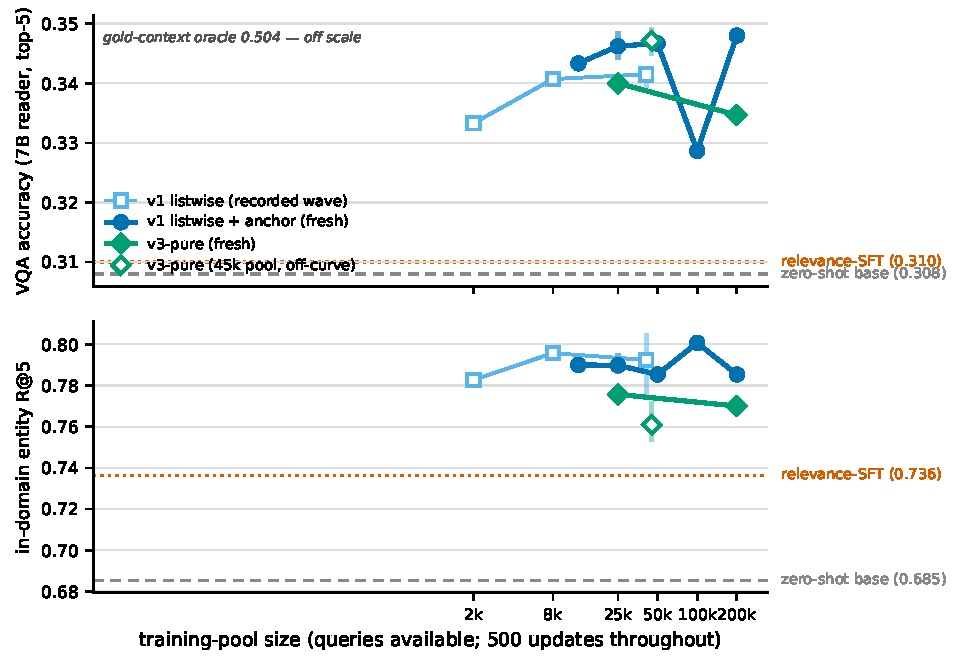
\includegraphics[width=0.72\textwidth]{fig_mm_scaling.pdf}
\caption{\textbf{The ceiling is a property of the recipe, not of the data budget.} Downstream
VQA accuracy of the frozen \textsc{Qwen2.5-VL-7B} reader (top-$5$) for \textsc{GME-Qwen2-VL-2B}
retrievers trained on nested InfoSeek query subsets at fixed compute ($500$ updates throughout).
Across a $16\times$ range of available training data the curve is flat to within $2$ points and
never approaches a data-limited regime, because at $500$ steps $\times$ batch $4$ only
${\sim}2{,}000$ queries are ever visited. \emph{Both ladder series are the v1 listwise recipe}
(anchored, deterministic top-$8$): filled circles are fresh same-cluster retrains, open squares
the pre-cluster-move recorded wave, shown separately because absolute levels are not comparable
across waves. The single \textsc{v3-pure} point is the headline three-seed cell at $45{,}248$
queries (all of \texttt{pool\_train}, a different and smaller pool file than the ladder's); the
matching v3 scaling cells are in flight, so \textbf{the data-scaling behaviour of the corrected
policy gradient is not yet measured} and no v3 curve should be read into this figure. Dashed
lines are the fresh zero-shot and relevance-SFT reproductions. Whiskers: seed min--max.}
\label{fig:mm_scaling}
\end{figure}

